%% Layout of a paper figure, filled by scripts/exporters/export_paper_figs.py: every %%PLOTS%% line is replaced by the
%% plots of one axis, in order. Lines starting with %% are dropped from the output.
\centering
% \begin{tabular}
% {@{}lll@{}}\tikz\draw[cyan!60!black, thick, mark=*, mark size=1.5] plot coordinates {(0,0) (0.4,0)}; {\small \model{gemma31}} & \tikz\draw[red!40, thick, mark=*, mark size=1.5] plot coordinates {(0,0) (0.4,0)}; {\small \model{llama8}} & \tikz\draw[yellow!60!black, thick, mark=*, mark size=1.5] plot coordinates {(0,0) (0.4,0)}; {\small \model{mistral24}}
% \end{tabular}\\[2pt]
% \begin{tabular}{@{}lll@{}}
% \tikz\draw[red!70!black, thick, mark=*, mark size=1.5] plot coordinates {(0,0) (0.4,0)}; {\small \model{olmo32}} & \tikz\draw[green!40!black, thick, mark=*, mark size=1.5] plot coordinates {(0,0) (0.4,0)}; {\small \model{qwen14}} & \tikz\draw[blue!70!black, thick, mark=*, mark size=1.5] plot coordinates {(0,0) (0.4,0)}; {\small \model{qwen32}}\end{tabular}\\[2pt]
% \begin{tabular}{@{}ll@{}}\tikz\draw[teal!70!black, thick, mark=*, mark size=1.5] plot coordinates {(0,0) (0.4,0)}; {\small \model{qwen27}} & \tikz\draw[brown!80!black, thick, mark=*, mark size=1.5] plot coordinates {(0,0) (0.4,0)}; {\small \model{seed36}}\end{tabular}\\[4pt]
%
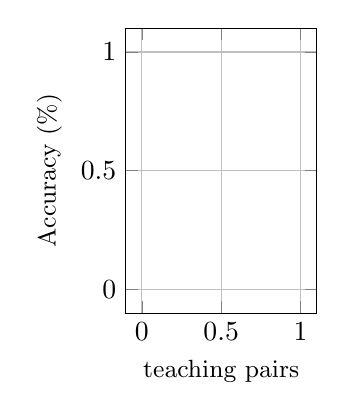
\begin{tikzpicture}[baseline=(current bounding box.center)]
\begin{axis}[
    height=5.2cm,
    width=4cm,
    grid=major,
    xlabel={\small teaching pairs},
    ylabel={\small Accuracy (\%)},
    xtick={0,1,3,5,7,9},
    legend entries={},
]
%%PLOTS%%
\end{axis}
\end{tikzpicture}
{ 
\small
\def\drawsymbol[#1]{\tikz\draw[#1,thick, mark=*, mark size=1.5] plot coordinates {(0,0) (0.4,0)};}
\begin{tabular}{@{}ll@{}}
\drawsymbol[cyan!60!black] &\model{gemma31} \\
\drawsymbol[red!40] &\model{llama8} \\
\drawsymbol[yellow!60!black] &\model{mistral24} \\
\drawsymbol[red!70!black] &\model{olmo32} \\
\drawsymbol[green!40!black] &\model{qwen14} \\
\drawsymbol[blue!70!black] &\model{qwen32} \\
\drawsymbol[teal!70!black] &\model{qwen27} \\
\drawsymbol[brown!80!black] &\model{seed36}
\end{tabular}
}
